\section{Die Überwindung der Rückständigkeit Deutschlands}
\label{sec:aufh-rueckst-d}
\index{Industrialisierung!Deutschland}

\begin{figure}
\centering
%\begin{sideways}
%\input{vergl-d-e.eepic}
%\end{sideways}
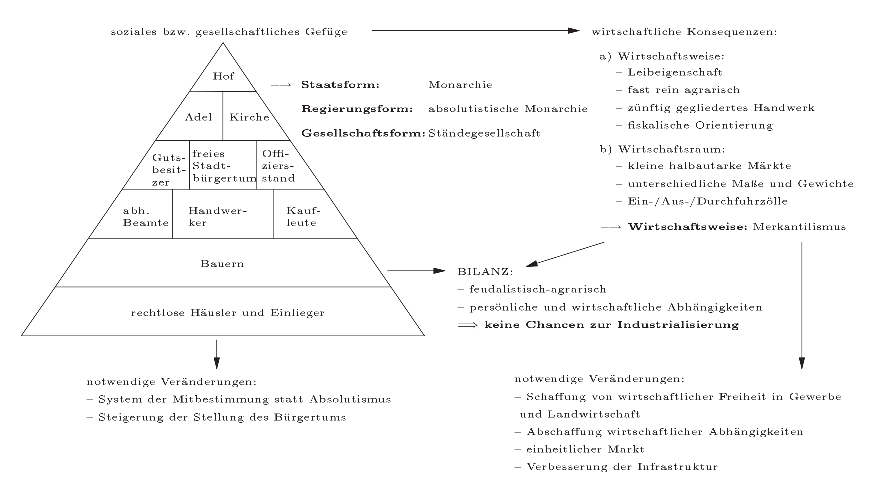
\includegraphics[width=\textwidth]{vergl-d-e.eps}
\caption{Die deutschen Verhältnisse}
\label{pic:dt-verh}
\index{Deutschland!Rückständigkeit}
\end{figure}

\begin{aufgabe}
Zeigen Sie an vier ausgewählten Faktoren, daß Deutschland im
Vergleich zu England als rückständig zu bezeichnen ist!
\end{aufgabe}

\paragraph{Wie Abbildung \ref{pic:dt-verh} zeigt,} waren um 1800
dringend Maßnahmen nötig, um ebenfalls in die industrielle Revolution
einsteigen zu können. Dieser Abschnitt soll zeigen, wie diese
beschaffen waren und was sie bewirkten. \\

\begin{aufgabe}
Stellen Sie an einem Beispiel die Überwindung der Rückständigkeit
Deutschlands im Vergleich zu England dar!
\end{aufgabe}

\subsection[Die Preußischen Reformen]
{Die Preußischen Reformen\footnote{Da die Informationen aus dem im
Geschichtsunterricht gehaltenen Vortrag ungeeignet waren, verwende ich
hier hauptsächlich Material aus \cite{BaswiSchuGesch}.}}
\index{Preußische Reformen}

\mar{Welche Idioten haben damals den Vortrag zu diesem Thema gemacht?}
\begin{aufgabe}
Untersuchen Sie die Preußischen Reformen auf ihre Veränderungen
für das Wirtschaftsgefüge hin!

Fassen Sie sämtliche Informationen zusammen, die zum wirtschaftlichen
Aufschwung Deutschlands als Voraussetzung anzusehen sind und stellen
Sie deren Wirkung dar!
\end{aufgabe}

\paragraph{Nach dem \dat{Krieg gegen Napoleon 1806/1807}} war Preußen
dem Zusammenbruch nahe. Daraufhin initiierten fortschrittliche und
einflußreichende Persönlichkeiten -- allen voran Reichsfreiherr
\Nam{Stein, Karl vom und zum}{Karl vom und zum Stein} und Fürst
\Nam{Hardenberg, Karl August von}{Karl August von Hardenberg} -- eine
Reihe von tiefgreifenden Reformen, die den Wiederaufbau und die
Befreiung des Staates von der französischen Fremdherrschaft
ermöglichen sollten.

Damit einher ging auch eine wirtschaftliche Reform Preußens, dessen
auf dem System der persönlichen Abhängigkeit beruhende Gutswirtschaft
von am Wirtschaftsliberalismus orientierten Grundsätze abgelöst
wurde.

\subsubsection{Bauernbefreiung}
\index{Bauernbefreiung}
\index{Regulierungsedikt}
\index{Oktoberedikt}

Das \dat{Oktoberedikt von 1807} hob die Erbuntertänigkeit und damit
die Leibeigenschaft auf und ermöglichte ihnen den Besitz von eigenem
Land. Die Gutsbesitzer wurden gemäß dem \dat{Regulierungsedikt von
1809} entschädigt.

Der so geschaffene \emph{freie Bauernstand} war nun in den
Wirtschaftsprozeß integriert und also an Produktionssteigerungen
interessiert.

\subsubsection{Städteordnung}
\index{Städteordnung}

Mit der \dat{Einführung der Städteordnung 1808} gewährte Preußen seine
Städten die selbständige Verwaltung ihrer Angelegenheiten. Die Bürger
konnten fortan aktiv und passiv an der an einen niedrigen Zensus
gebundenen Wahl zur Stadtverordnetenversammlung, die
wiederum Magistrat und Bürgermeister (Exekutive) wählte, teil- und
damit auf die Politik Einfluß nehmen.

Dies sind die Ursprünge der kommunalen Selbstverwaltung in Deutschland.

\subsubsection{Verwaltungsreform}
\index{Verwaltungsreform}

Die \emph{Verwaltungsreform} sollte
\textquote[\cite{BaswiSchuGesch}]{einen lestungsfähigen, sparsamen
und bürgernahen Staatsapparat [\dots] schaffen.} Dazu gehörten eine
Vereinfachung der Behördenstruktur durch eindeutige Klärung der
Zuständigkeiten und die Trennung von Justiz und Verwaltung. Möglich
wurde dies durch die neuen Ein"-stel"-lungs- und Laufbahnkriterien für
Beamte (Qualität statt Gunst) und die fortschreitende
Verschriftlichung und Archivierung von Vorgängen. -- Das
Berufsbeamtentum, wie es heute noch fast unverändert in Deutschland
besteht, wurde geprägt. -- Außerdem wurden die Beamten durch relativ
hohe Gehälter bestechungssicher gemacht.\mycite{WikPreusRef}

Ein weiterer bedeutender Inhalt der Verwaltungsreform war die
Schaffung des \emph{klassischen Kabinetts} aus Ministerien (fünf an
der Zahl) mit klar abgegrenzten Ressorts.

\subsubsection{Gewerbereform}
\index{Gewerbereform}

\dat{1810/11 wurde die Gewerbefreiheit} eingeführt. -- Um ein Gewerbe
aufzunehmen genügte der Erwerb eines Gewerbescheins.
\mar{Gewerbe\-steuer? -- Stimmt. Einfügen!} Damit ging die Aufhebung
des Zunftzwangs und somit die Beseitigung zahlreicher Monopole einher.
Dies und die weitgehende Abschaffung der staatlichen Aufsicht über die
Wirtschaft beförderte Konkurrenz und freien Markt.

\subsubsection{Folgen}

\begin{itemize}
\item Unabhängigkeit von den Gutsherren bringt ehemalige Bauern als
Arbeitskräfte in die Städte.
\item zunehmende Bedeutung des Gewerbes auch in ländlichen Gebieten
\item zunehmende Verstädterung
\item später: Verschärfung der sozialen Frage durch übermäßige Zunahme
der Zahl der Handwerker bei starker Konkurrenz
\end{itemize}


%%%%%%%%%%%%%%%%%%%%%%%%%%%%%%%%%%%%%%%%%%%%%%%%%%%%%%%%%%%%%%%%%%%%%%

\subsection{\dat{Die Fr"uhindustrialisierung 1770\,--\,1850}}
\label{ssc:frueh-ind}
\index{Fr"uhindustrialisierung}

\begin{aufgabe}
Stellen Sie Ansätze wirtschaftlichen Aufschwunges in Deutschland
anhand der Frühindustrialisierung dar!

Bewerten Sie die Wirkungsweise dieser auf den
Industrialisierungsprozeß insgesamt!
\end{aufgabe}

\paragraph{Die Verarbeitung von Agrarprodukten} wie sie in
Zuckerfabriken, Branntweinbrennereien, Brauereien, Ölmühlen und
Tabakfabriken betrieben wurde, bildete die Wurzeln des
Unternehmertums. So wurde beispielsweise der Zuckerrübenbauer zum
Zuckerfabrikanten und der Textilverleger zum Textilfabrikanten.

\paragraph{Die Textilproduktion beruhte auf dem Verlagssystem}
(beispielsweise heimgewerbliche Leinenherstellung), das in dieser
Phase der Industrialisierung zur Blüte kam
\mycite[207]{gelbesGeschichts}.  Mit der \dat{Einführung mechanischer
Webstühle 1830} wurden dann die Voraussetzungen für die
Textilindustrie geschaffen.

\paragraph{Ferner erschloß man neue Industriezweige,} wie den
Kohlebergbau und die Erzgewinnung.\\

Diese Ansätze wirtschaftlichen Aufschwungs schufen einen Bedarf nach
Maschinen. -- Kleine Reparaturwerkstätten entwickelten sich zu
Maschinenfabriken. -- Man benötigte Metall. -- Um die isolierten
Produktionsinseln zu verbinden, mußte man die Infrastruktur aufbauen.
-- Man baute 1835 die erste Eisenbahnstrecke. -- Wieder brauchte man
Metall.

Hier zeigen sich die Grundlagen der \beg{Interdependenzen} -- starker
Rückkopplungseffekte, die die folgende rasante Entwicklung
Deutschlands vom Agrar- zum Industriestaat bedingten.

Die Wirtschaft selber entwickelte sich in der Zeit der
Frühindustrialisierung allerdings nur langsam.

%%%%%%%%%%%%%%%%%%%%%%%%%%%%%%%%%%%%%%%%%%%%%%%%%%%%%%%%%%%%%%%%%%%%%%

\subsection{Der Zollverein}
\label{ssc:zollv}
\index{Zollverein}

\begin{aufgabe}
Stellen Sie den Entstehungsprozeß des Zollvereins dar!

Bewerten Sie seine Bedeutung für den Wirtschaftsaufschwung/die
Industrialisierung in Deutschland!
\end{aufgabe}

\subsubsection{Entstehungsprozeß}

\paragraph{Vorläufer:} süddeutscher Zollverein, mitteldeutscher
Handelsverein, preußisch-hessischer Verein

\begin{chronik}
\item[1.\,1.\,1834]
\dat{Zollvereinigungsvertrag} zwischen den Vorläufervereinen -- Der
\emph{deutsche Zollverein} entsteht.

\item[bis 1854]
Westerweiterung durch Anschluß weiterer Länder

\item[1857]
Einführung des Zollvereinstalers

\item[1867]
Norderweiterung

\item[1868]
verbindliche Einführung von \emph{Meter und Kilogramm}
\index{metrisches System}

\item[1871]
Zollverein ist vollständig\footnote{Zur Zusammensetzung des
Zollvereins siehe
\href{http://de.wikipedia.org/wiki/Gebiet_des_Deutschen_Zollvereins}
{diesen Wikipediaartikel}}
\footnote{Österreich wurde trotz Antrages nicht aufgenommen, da das
den Verein dominierende Preußen seine Rivale durch die zusätzlichen
Zahlungen schwächen konnte.}
und umfaßt zur Reichsgründung das gesamte Reichsgebiet
\index{Deutsches Reich}
\end{chronik}


\subsubsection{Politische Bedeutung}

\begin{itemize}
\item ökonomische und materielle Verbindung der Deutschen zu einer
\emph{Nation}
\item Vorbereitung einer echten Nation
\item Stärkung der materiellen Kraft der deutschen Lande durch Wahrung
der auswärtigen Gesamtinteressen
\item Verschmelzung einzelner Provinzialinteressen zu einem
Nationalinteresse -- Erweckung eines Nationalgefühls
\end{itemize}

\subsubsection{Wirtschaftliche Bedeutung}

\begin{itemize}
\item \mar{?} Wiedergeburt des deutschen Unternehmergeistes
\item \mar{?} Teilhabe der deutschen an allen
Nationalangelegenheiten 
\item \mar{?} Anteilnahme des Mittelstandes und der
Großgrundbesitzer an praktischer Politik
\item Grundlage für einheitlichen Markt
\item Wegfall der Zollschranken
\item einheitliche Währung und Maßeinheiten
\end{itemize}

$\Longrightarrow$ Bedingung für ein modernes Wirtschaftssystem


%%%%%%%%%%%%%%%%%%%%%%%%%%%%%%%%%%%%%%%%%%%%%%%%%%%%%%%%%%%%%%%%%%%%%%

\subsection{Der neue Unternehmertypus}
\index{Deutschland!Unternehmertum}

\begin{aufgabe}
Zeigen Sie, daß sich in Deutschland ein neuer Unternehmertypus
Herausbildete und stellen Sie ihn vor!

Begründen Sie, daß er einen Beitrag zur Überwindung der
Rückständigkeit Deutschlands leisten konnte!
\end{aufgabe}

\subsubsection{Entstehung von Unternehmen}

\begin{itemize}
\item Handwerker bauen auf technischen oder finanziellen Grundlagen
oder auf Basis einer Idee Werkstätten zu Fabriken aus.
\item \beg{Feudalunternehmer}
\item Unternehmensgründung auf Basis von Kapitalbesitz oder Erbschaft
(z.\,B. \Nam{Krupp, Alfred}{Alfred Krupp}
\end{itemize}

\subsubsection{Entwicklung zum \emph{neuen} Unternehmer}

Private Unternehmer, Techniker, Kaufleute, Wissenschaftler und
Politiker unternahmen Bildungsreisen nach Großbritannien, von wo sie
Technologien und Anregungen für das deutsche Bildungswesen
mitbrachten. Sie importierten auch britische Maschinen und knüpften
Beziehungen, über welche sie britische Fachleute nach Deutschland
holten.

Hier entwickelte sich eine neue Art, Unternehmen zu gründen: Man
setzte risikofreudig teilweise das gesamte Eigen- oder auch
Familienkapital ein. Wo dieses nicht reichte, schlossen sich mehrere
Unternehmer zusammen -- man gründete Aktiengesellschaften -- oder
wurden Kredite aufgenommen -- Großbanken, wie die \ins{Deutsche Bank}
oder die \ins{Dresdner Bank} entstanden.

\subsubsection{Mitwirkung der Unternehmer bei der Überwindung der
Rückständigkeit Deutschlands}

\begin{description}
\item[Wissen und Erfahrung:] Import von technischen Neuerungen,
Maschinen, Facharbeitern und Ingenieuren
\item[Bildungssystem:] Übergang zu innerdeutscher Ausbildung von
Fachkräften und Ingenieuren an Fachschulen und technischen Hochschulen
\item[Aufschwung des Finanzwesens:] hohe private Investitionen und
damit verbundenes Risiko
\item[technischer Fortschritt:] Kapitalismus führt zu hohem
Konkurrenzdruck -- Unternehmen verbessern eigenständig Produktions-
und Verarbeitungsprozesse. (forschendes Unternehmertum)
\end{description}

Damit war bald sowohl die finanzielle wie auch die technologische
Unabhängigkeit vom Ausland gewährleistet. Die neuen Unternehmer trugen
so maßgeblich zum Aufbau eines wirtschaftlich konkurrenzfähigen
deutschen Kaiserreiches bei.

%%%%%%%%%%%%%%%%%%%%%%%%%%%%%%%%%%%%%%%%%%%%%%%%%%%%%%%%%%%%%%%%%%%%%%

\subsection[Veränderungen in der Infrastruktur]
{Veränderungen in der Infrastruktur \mycite[157/158]{braunesGeschichts}}

\begin{aufgabe}
Weisen Sie nach, daß eine Verbesserung der Infrastruktur in
Deutschland stattgefunden hat!

Bewerten Sie die Bedeutung dessen für den Industrialisierungsprozeß!
\end{aufgabe}

\paragraph{Die Verbesserung der deutschen Infrastruktur} begann in der
Zeit der Frühindustrialisierung: Man befestigte die Landstraßen, baute
Flüsse aus und verband sie durch Kanäle. Dampfschiffe erleichterten
und beschleunigten den den Gütertransport.

\paragraph{Die weitaus bedeutendste Veränderung} war aber die
Einführung der Eisenbahn \index{Eisenbahn} in Deutschland. Nur
sinnvoll durch den Zollverein (\emph{siamesische Zwillinge}) erfuhr
sie seit ihrem \dat{ersten Einsatz 1935} eine rasante
Entwicklung\footnote{Zu konkreten Zahlen siehe
\cite[159]{braunesGeschichts} und \cite{WikEisenbahn}} und wurde zum
entscheidenden Motor der Industrialisierung.

Einerseits erleichterte, beschleunigte und verbilligte sie den
Personen- und Warenverkehr erheblich. Dadurch eröffneten sich nicht
nur neue Möglichkeiten, Rohstoffe zu beschaffen beziehungsweise
Produkte zu vertreiben, sondern förderte ebenso den kulturellen
Austausch und vergrößerte die Anzahl der Arbeiter in Form von
Pendlern.

Andererseits befeuerte die neue riesige Nachfrage nach Stahl für
Schienenverlegung und Eisenbahnherstellung die Schwerindustrie und den
Arbeitsmarkt. Deren Expansion verlangte wiederum nach weiterem Ausbau
der Eisenbahn und so weiter. -- Diese äußerst starke
\beg{Interdependenz} führte in der Folge den sprunghaften Anstieg der
Wirtschaftsmacht Deutschlands.



%%%%%%%%%%%%%%%%%%%%%%%%%%%%%%%%%%%%%%%%%%%%%%%%%%%%%%%%%%%%%%%%%%%%%%

\subsection{Entstehung von Industriegebieten -- Das Ruhrgebiet}
\index{Industriegebiete!Entstehung}
\index{Ruhrgebiet}

\begin{aufgabe}
Zeigen Sie am Beispiel des Ruhrgebietes die schrittweise Entstehung
industrieller Ballungsgebiete!

Bewerten Sie die Bedeutung solcher Ballungsgebiete für den
Industrialisierungsprozeß!
\end{aufgabe}

\subsubsection[Entstehungsprozeß]{Entstehungsprozeß\footnote{Hier am
Beispiel des Ruhrgebiets. -- In anderen Gebieten ähnlich.}}

\begin{enumerate}
\item heranwachsende Stahlindustrie seit 1820 -- Strukturwandel von
Landwirtschaft zu Industrie nach Kohlefunden
\item 1840\,--\,1848 Ausbau von Eisenbahn und Binnenschiffahrt führt
zur Verbesserung der Infrastruktur
\item Übergang vom Stollen- zum Schachtbau
\item Eröffnung von Zechen in großer Zahl führt zu starker Zuwanderung
\item Eisenindustrie ab 1850, forcierte Entwicklung durch Eisenbahnbau
\item 1850\,--\,1870: Kohle!
\item Land- und Intensivwirtschaft zur Versorgung der Bevölkerung in
den Randgebieten der Ballungszentren
\item Nachfolgeindustrien
\end{enumerate}

\subsubsection{Bedeutung der Ballungsgebiete für den
Industrialisierungsprozeß}

\begin{itemize}
\item kein Zoll
\item kürzere Transportwege
\item Zusammenarbeit der Unterhehmen
\item Konzentration von Fachpersonal
\item Konzentration von Wissenschaft und Forschung
\item Investition der Rendite in neue Techniken, Betriebe etc.
\end{itemize}

$\Longrightarrow$ Sprungbrett für die Industrialisierung des gesamten
Landes

\endinput
